\documentclass[french]{beamer}
\usepackage{comment}
\usepackage[utf8]{inputenc}
\usepackage[T1]{fontenc}
\usepackage{lmodern}
\usepackage{amsmath, amssymb}
\usepackage{multimedia}
\usepackage{babel}
\usepackage{pgfplots}
\usetheme[width=2cm]{PaloAlto}
\usepackage{graphicx}
\usepackage{textpos}
\usepackage{mathrsfs}
\usetikzlibrary{patterns}
\pgfplotsset{compat=1.15}
\usetikzlibrary{arrows}
\usepackage{multimedia}
\usepackage{pdfpages}
\usepackage{algorithm}
\usepackage{algorithmic}
\title{Automated Anomaly Detection in Large Sequences}
\subtitle{ Paul Boniol, Michele Linardi, Federico Roncallo, Themis Palpanas}
\author{ Grégoire Béchade \\ Alexis Marouani}
\date{19 Décembre 2024}




\begin{document}

\begin{frame}
	\titlepage
\end{frame}


\begin{frame}{Introduction and context}
    Classical anomaly detection methods rely on comparing a subsequence to each other subsequence in the time-series. \\
    It raises problems when facing : 
    \begin{itemize}
        \item Large time-series
        \item Repeated anomalies\\[0.5cm]
    \end{itemize}

    \begin{figure}
        \centering
        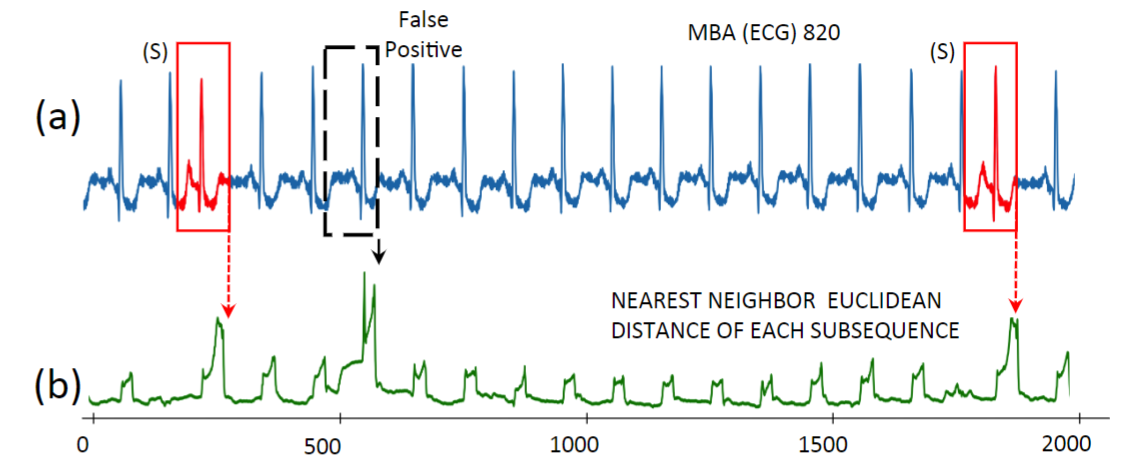
\includegraphics[width=0.7\textwidth]{heartbeats.png}
        \caption{Heartbeats with several anomalies}
    \end{figure}
    
\end{frame}

\begin{frame}{Method}
    The article introduces a new method to perform anomaly detection in large time series, which relies on the introduction of a "normal behaviour" of the time series.\\[1cm]
    \begin{exampleblock}{Construction of $N_M$}
        \begin{itemize}
            \item Randomly select subsequences of length $3 \times l$
            \item Hierarchical clustering of the subsequences
            \item Select the cluster $c$ that maximises $N(c) = \frac{frequency (c)^2 \times coverage (c) }{ \Sigma_{x \in \mathbb{C} } dist(center(c), center(x))}$
        \end{itemize}
    

    \end{exampleblock}
\tiny{Idea : The normal cluster is the one that is the most frequent and the most central.}
    
\end{frame}

\begin{frame}{Method}
\textbf{Outliers detection :} 

For each subsequence of size $l$ in the time series : 
\begin{itemize}
    \item Compute the distances to all subsequences of size $l$ in $N_M$. 
    \item Label as anomalies the k sequences with the largest distance to $M_N$, or the one that are above a certain threshold.
\end{itemize}

\end{frame}


\end{document}


%% Mise en page:
%\begin{minipage}{0.4\linewidth}
%\end{minipage}\hfill 
%\begin{minipage}{0.4\linewidth}
%\begin{exampleblock}{Résultats}
%% Pour les images:
%\includegraphics[height=4cm]{image/7.pdf}

 
